
\documentclass[hyperref={breaklinks=true},fleqn,mathserif]{beamer}
%\documentclass[draft,hyperref={breaklinks=true},fleqn,mathserif]{beamer}

% Spausdinimui ant popieriaus:
%\documentclass[hyperref={breaklinks=true},fleqn,mathserif,handout]{beamer}
%\usepackage{pgfpages}
%\pgfpagesuselayout{4 on 1}[a4paper,landscape,border shrink=5mm]

\usepackage{algorithmic}

%%%%%%%%%%%%%%%%%%%%%%%%%%%%%%%%%%%%%%%%%%%%%%%%%%%%%%%%%%%%%%%%%%%%%%%%%%%%%%%%
% SI units
\usepackage{siunitx}
%\sisetup{detect-all}
%%%%%%%%%%%%%%%%%%%%%%%%%%%%%%%%%%%%%%%%%%%%%%%%%%%%%%%%%%%%%%%%%%%%%%%%%%%%%%%%

%%%%%%%%%%%%%%%%%%%%%%%%%%%%%%%%%%%%%%%%%%%%%%%%%%%%%%%%%%%%%%%%%%%%%%%%%%%%%%%%
\usepackage[utf8x]{inputenc} % atkomentuoti, jei naudojat utf-8 koduotę
\usepackage[L7x]{fontenc}
\usepackage[english,lithuanian]{babel}
%%%%%%%%%%%%%%%%%%%%%%%%%%%%%%%%%%%%%%%%%%%%%%%%%%%%%%%%%%%%%%%%%%%%%%%%%%%%%%%%

\usetheme{Warsaw}
%\usecolortheme{beaver}

% Pašalina Navigation Bar
\setbeamertemplate{navigation symbols}{}

\setbeamersize{text margin left=1em,text margin right=1em}

%\setbeamertemplate{footline}[page number]

%\AtBeginSection[]
%{
%\begin{frame}
%    \frametitle{Turinys}
%    \tableofcontents[currentsection]
%\end{frame}
%}

%\AtBeginSubsection[]
%{
%\begin{frame}
%    \frametitle{Outline}
%    \tableofcontents[currentsection,currentsubsection]
%\end{frame}
%}

\title[Modeling of Multilayer Biosensor]{Numerical Modeling of Multilayer Biosensor with Degrading Substrate and Product}
%\subtitle{Papildomas subtitle}
\author[Tadas Meškauskas \textit{et al.}]{\textbf{\underline{Tadas Me\v{s}kauskas}${}^{*}$, Feliksas Ivanauskas${}^{*}$ and \\ Valdas Laurinavi\v{c}ius${}^{\ddag}$}}
\institute{Vilnius University, Lithuania \\
    \smallskip ${}^{*}$Faculty of Mathematics and Informatics \\
    ${}^{\ddag}$Vilnius University Institute of Biochemistry \\
    \smallskip e-mail: \textit{tadas.meskauskas@mif.vu.lt} \\
}
\date{{\scriptsize EUROSIM2013 -- $8^{th}$ EUROSIM Congress on Modelling and Simulation \\
    (Cardiff, Wales, United Kingdom, 10-12 September 2013)}
}

% slide numbering in Beamer class (Warsaw theme), pagal http://tex.stackexchange.com/questions/8179/slide-numbering-in-beamer-class-warsaw-theme
\defbeamertemplate*{footline}{shadow theme}
{%
    \leavevmode%
    \hbox{\begin{beamercolorbox}[wd=.5\paperwidth,ht=2.5ex,dp=1.125ex,leftskip=.3cm plus1fil,rightskip=.3cm]{author in head/foot}%
    \usebeamerfont{author in head/foot}\insertframenumber\,/\,\inserttotalframenumber\hfill\insertshortauthor
    \end{beamercolorbox}%
    \begin{beamercolorbox}[wd=.5\paperwidth,ht=2.5ex,dp=1.125ex,leftskip=.3cm,rightskip=.3cm plus1fil]{title in head/foot}%
    \usebeamerfont{title in head/foot}\insertshorttitle%
    \end{beamercolorbox}}%
    \vskip0pt%
}

\newcommand*{\urlw}[1]{\href{#1}%
            {\nolinkurl{#1}}}

\newcommand{\St}{\frac{\partial S}{\partial t}}
\newcommand{\Sx}{\frac{\partial S}{\partial x}}
\newcommand{\SDxx}{\frac{\partial}{\partial x}\!\left(\!D_S(x)\Sx\right)}
\newcommand{\Pt}{\frac{\partial P}{\partial t}}
\newcommand{\Px}{\frac{\partial P}{\partial x}}
\newcommand{\PDxx}{\frac{\partial}{\partial x}\!\left(\!D_P(x)\Px\right)}
\newcommand{\xim}{x_{i-\frac12}}
\newcommand{\xip}{x_{i+\frac12}}
\newcommand{\NMV}{N\!-\!1}


\begin{document}

%\frame[plain]{\titlepage}
%\frame{\titlepage}

\frame[plain]{\titlepage}
%\frame{\titlepage}

\begin{frame}
    \frametitle{Outline}
    \tableofcontents[section,subsection]
\end{frame}

%%%%%%%%%%%%%%%%%%%%%%%%%%%%%%%%%%%%%%%%%%%%%%%%%%%%%%%%%%%%%%%%%%%%%%%%%%%%%%%%
\section{Model of multilayer biosensor}
%%%%%%%%%%%%%%%%%%%%%%%%%%%%%%%%%%%%%%%%%%%%%%%%%%%%%%%%%%%%%%%%%%%%%%%%%%%%%%%%

\subsection{Electrochemical biosensor}

%%%%%%%%%%%%%%%%%%%%%%%%%%
\begin{frame}[shrink=17]{Principal scheme of electrochemical biosensor}
%\frametitle{Principal scheme of electrochemical biosensor}

\begin{block}{As a model device, an electrochemical biosensor is dealt with}
Enzyme catalyzes conversion of substrate ($S$), which is our target, to product ($P$), which is electrochemically active and can be detected on the electrode:
\end{block}

\pause
\medskip
\centering{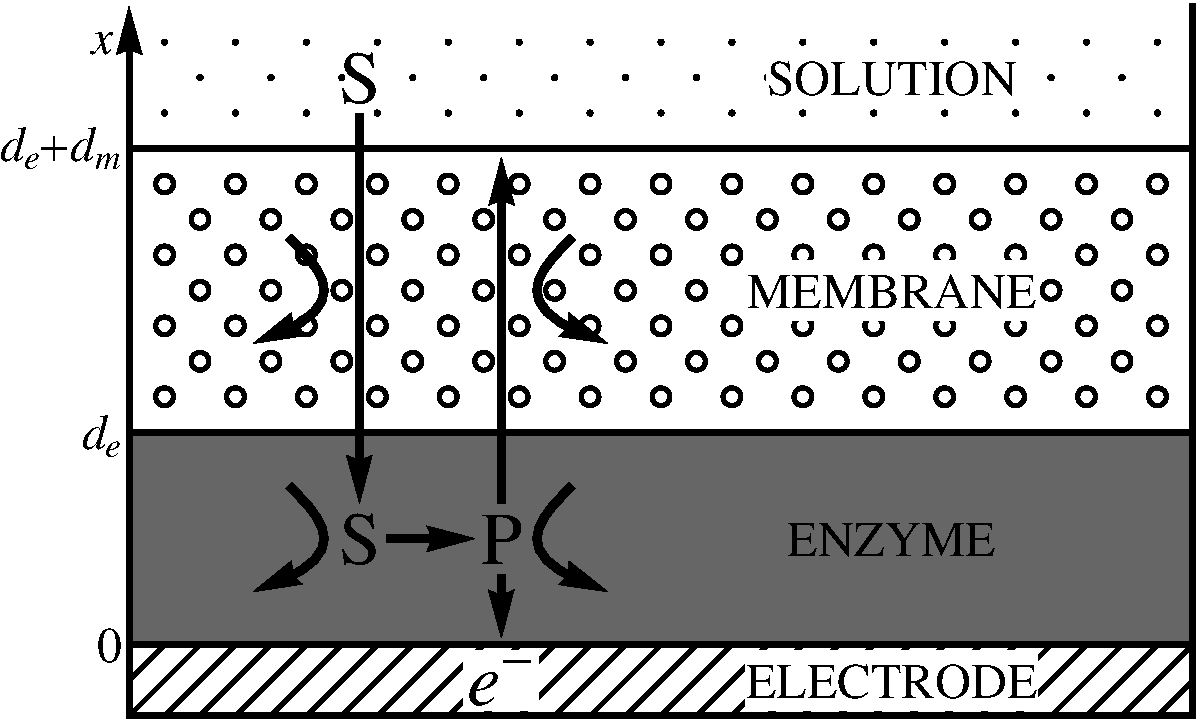
\includegraphics[clip=true, width=70mm]{Iliustracijos/Fig1.pdf}\\
Mathematical variable $x$ denotes distance to the electrode.
}

\pause
\begin{exampleblock}{}
Current on the electrode defines {\color{blue} \emph{the response}} of the biosensor.

The same principal scheme can be applied to optical, electromagnetic and a number of other biosensors.
\end{exampleblock}

\end{frame}
%%%%%%%%%%%%%%%%%%%%%%%%%%

%%%%%%%%%%%%%%%%%%%%%%%%%%
\begin{frame}[shrink=11]{Impact of unstable substrate and product?}

\centering{
\begin{minipage}{0.48\textwidth}
    \smallskip
    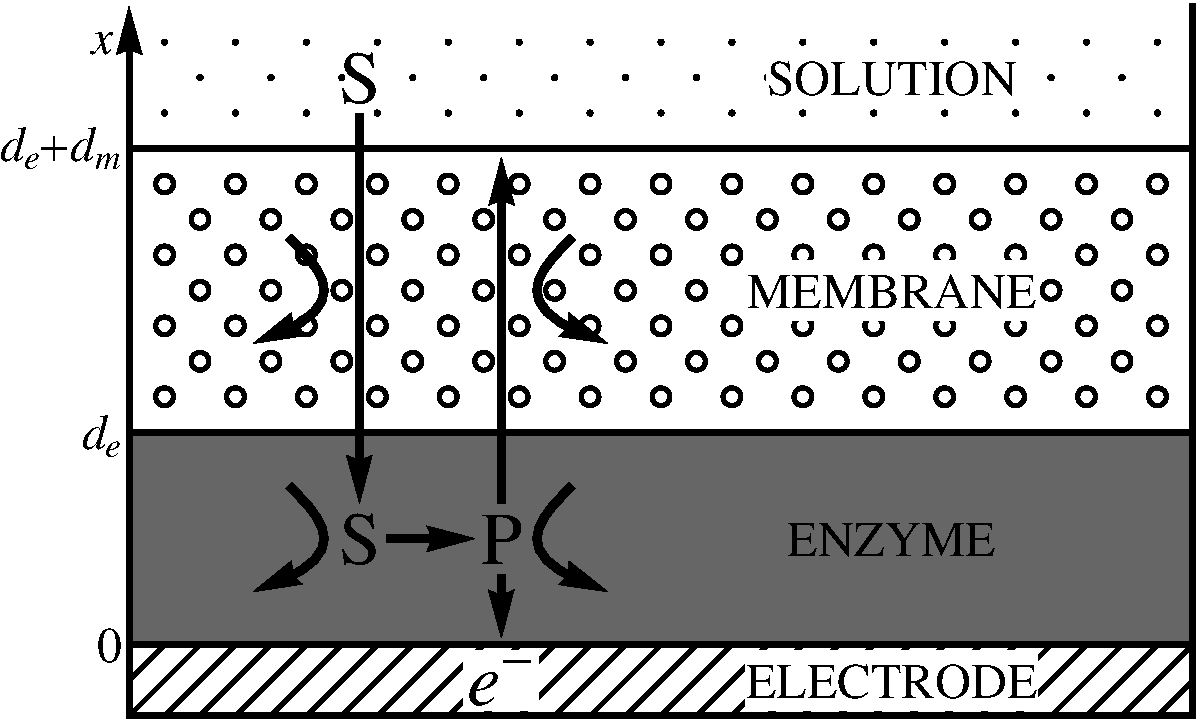
\includegraphics[clip=true, width=\textwidth]{Iliustracijos/Fig1.pdf}
\end{minipage}
\;
\begin{minipage}{0.48\textwidth}
    \begin{alertblock}{How degrading substrate and/or product will influence on the response of the biosensor?}
    Often substrate and/or product is consumed by extraneous enzymes, microorganisms, spontaneous decomposition or other side reactions.

    \smallskip
    How parameters of the biosensor will affect this influence?
    \end{alertblock}
\end{minipage}
}

\pause
\begin{block}{}
For estimation of the influence of creep processes we are going to propose a mathematical algorithm and biosensor response correcting formulae.

\smallskip
Evaluation of creep processes in biosensors will predict limiting conditions of the biosensor application and improve the reliability of the biosensors
that is necessary implementing biosensors in the automated monitoring processes in industry, environment control and medicine.
\end{block}

\end{frame}
%%%%%%%%%%%%%%%%%%%%%%%%%%

\subsection{Mathematical model}

%%%%%%%%%%%%%%%%%%%%%%%%%%
\begin{frame}[shrink=20]{Differential equations}

\vspace*{-3mm}
\begin{block}{Action of the enzyme will be expressed as a Michaelis--Menten process.}
It means that we accept conditions, when concentration of the product $P$ inside the enzyme containing membrane will be lower than concentration of the substrate $S$.
In the steady-state conditions this requirement can be realized when the rate of $P$ consumption on the electrode surface will be sufficiently fast.
\end{block}

\vspace*{-6mm}
\begin{gather*}
    \St  =  \SDxx  -  C_1 S  -  \alpha(x) \frac{V_{max}\, S}{K_M + S}, \\
    \Pt  =  \PDxx  -  C_2 P  +  \alpha(x) \frac{V_{max}\, S}{K_M + S}, \qquad \mbox{here}
\end{gather*}

\pause
\vspace*{-5mm}
\centering{
\begin{minipage}{0.49\textwidth}
    \begin{gather*}
        D_S(x)  =
        \begin{cases}
            \,D_{S_e}, & 0 < x \leqslant d_e, \\
            \,D_{S_m}, & d_e < x < d_e + d_m,
        \end{cases} \\
        D_P(x)  =
        \begin{cases}
            \,D_{P_e}, & 0 < x \leqslant d_e, \\
            \,D_{P_m}, & d_e < x < d_e + d_m,
        \end{cases} \\
        \alpha(x)  =
        \begin{cases}
            \,1, & 0 < x \leqslant d_e, \\
            \,0, & d_e < x < d_e + d_m,
        \end{cases}\phantom{x}
    \end{gather*}
\end{minipage}
\begin{minipage}{0.49\textwidth}
    \begin{exampleblock}{Parameters}
    Thicknesses of layers $d_e$ and $d_m$.

    Diffusion coefficients $D_{S_e}$, $D_{P_e}$, $D_{S_m}$, $D_{P_m}$.

    Substrate and product \emph{degradation} rate constants $C_1$ and $C_2$.

    $V_{max}$ is the maximum rate of the enzymatic reaction, $K_M$ represents the Michaelis constant.
    \end{exampleblock}
\end{minipage}
}

\end{frame}
%%%%%%%%%%%%%%%%%%%%%%%%%%

%%%%%%%%%%%%%%%%%%%%%%%%%%
\begin{frame}[shrink=21]{Biosensor parameters}

\begin{block}{}
As a model electrode -- glucose oxidase immobilized on Pt electrode has been applied.
Current of hydrogen peroxide electrochemical oxidation has been recorded.
In numerical experiments activity of immobilized glucose oxidase has been accepted to be $V_{max} ={}$\SI{0.3}{\milli\mole\per\metre\cubed\per\second},
that is about three times lower than activity of native enzyme, taking into account that under immbolization process enzyme can loss $2/3$ of the initial activity.
$K_M$ of glucose oxidase from \textit{Aspergillus niger} is \SI{0.23}{\mole\per\metre\cubed} and it has been assumed that during the immobilization procedure
this parameter is not influenced.

\smallskip
Numerical experiments have been performed at $S_0 ={}$\SI{0.07}{\mole\per\metre\cubed} (concentration of substrate in buffer solution) as default.
It is approximately $3.3$ times lower than $K_M$, \textit{i.\,e.} biosensor operates in linear diapason of substrate.
\end{block}

\pause
\begin{exampleblock}{}
Layer of immobilized enzyme has been covered with acetylated cellulose film (outer membrane).
It is typical biosensor reported in many papers.

\smallskip
Thicknesses of layers $d_e ={}$\SI{9}{\micro\metre}, $d_m ={}$\SI{10}{\micro\metre}.
\end{exampleblock}

\pause
\begin{block}{}
Diffusion coefficients have been adjusted in accordance with experimental biosensor response curves:
$D_{S_e} ={}$\SI{22}{\micro\metre\squared\per\second}, $D_{P_e} ={}$\SI{20}{\micro\metre\squared\per\second},
$D_{S_m} ={}$\SI{7}{\micro\metre\squared\per\second}, $D_{P_m} ={}$\SI{6}{\micro\metre\squared\per\second}. 
\end{block}

\end{frame}
%%%%%%%%%%%%%%%%%%%%%%%%%%

%%%%%%%%%%%%%%%%%%%%%%%%%%
\begin{frame}[shrink=27]{Initial values and boundary conditions}

\begin{exampleblock}{Initial values}
At the beginning ($t=0$) there is no substrate ($S=0$), nor product ($P=0$) inside the enzymatic layer and the outer membrane:
\begin{gather*}
    S( x, 0 )  =
    \begin{cases}
        \,0,   & 0 \leqslant x < d_e + d_m, \\
        \,S_0, & x = d_e + d_m,
    \end{cases} \\
    P( x, 0 )  =  0,  \quad
    0 \leqslant x \leqslant d_e + d_m.\phantom{lxx}
\end{gather*}
\end{exampleblock}

\pause
\begin{block}{Boundary conditions}
Substrate is electrochemically inactive substance.
The rate of electrochemical conversion of product is very fast in compare with enzymatic reaction rate.
Hence, on the biosensor electrode ($x=0$) boundary conditions apply (for $t>0$):
\[
    \left. \Sx \right|_{x=0}  =  0,  \qquad
    P( 0, t )  =  0,  \qquad  t > 0.
\]

Another boundary condition defines $S$ values at the biosensor border ($x = d_e + d_m$) with buffer solution:
\[
    S( d_e\!+\!d_m, t )  =  S_0,  \qquad  t > 0.
\]
\end{block}

\end{frame}
%%%%%%%%%%%%%%%%%%%%%%%%%%

%%%%%%%%%%%%%%%%%%%%%%%%%%
\begin{frame}{Boundary conditions}

\begin{block}{We have examined two different options}
The first one assumes situation when {\color{blue} \emph{product diffuses out of the biosensor}}:
\[
    P( d_e\!+\!d_m, t )  =  0,  \qquad  t > 0.
\]

\pause
Alternatively, we can assume that {\color{blue} \emph{the outer membrane is not permeable}} for product $P$.
In this case $P$ is trapped inside the biosensor.
However, substrate permeability is the same as in the first case.
Such a situation can happen when both the product and the outer membrane are charged.
This implies the boundary condition
\[
    \left. \Px \right|_{x=d_e+d_m}  =  0,  \qquad  t > 0.
\]
\end{block}

\end{frame}
%%%%%%%%%%%%%%%%%%%%%%%%%%

\subsection{Numerical algorithm}

%%%%%%%%%%%%%%%%%%%%%%%%%%
\begin{frame}[shrink=8]{Crank--Nicolson difference scheme}

\begin{exampleblock}{}
The differential model has been approximated by {\color{blue} \emph{the Crank--Nicolson method}} (a second-order implicit finite difference scheme).

\smallskip
For each discrete time layer $t_k$, the resulting nonlinear system of algebraic equations can be solved iterating by the nonlinear part
and using {\color{blue} \emph{the Thomas algorithm}} (also known as the tridiagonal matrix algorithm) for the linear part.
\end{exampleblock}

\pause
\begin{block}{Grids in space and time directions}
The mathematical variables $x$ and $t$ are replaced by introducing grids (discrete values of variables).

\smallskip
Denote $\Omega_h$ the grid for the variable $x$ and $\omega_{\tau}$ the grid for the variable $t$.
\end{block}

\pause
\begin{exampleblock}{Computer implementation}
C programming language with MPI (Message Passing Interface) for communications between nodes (cores, processors).
\end{exampleblock}

\end{frame}
%%%%%%%%%%%%%%%%%%%%%%%%%%

%%%%%%%%%%%%%%%%%%%%%%%%%%
\begin{frame}{Uniform or non-uniform grids?}

\begin{alertblock}{}
The diffusion coefficients $D_S(x)$ and $D_P(x)$ are discontinuous at the junction point (of the enzymatic layer and the outer membrane) $x=d_e$.

\smallskip
Also, the initial values (when $t=0$) of the substrate concentration are discontinuous at the point $x = d_e + d_m$ (where the outer membrane meets the buffering solution).

\smallskip
Therefore, it may be intuitively expected that \emph{non-uniform} grids better suits the problem under investigation.
\end{alertblock}

\medskip
\centering{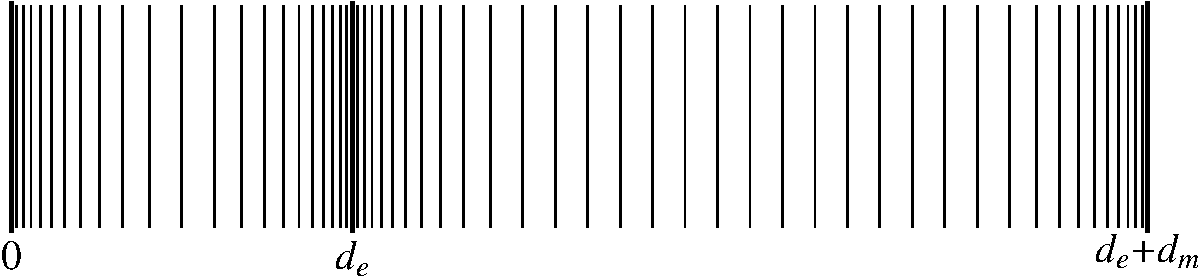
\includegraphics[clip=true, width=0.8\textwidth]{Iliustracijos/Fig_Netolygus_Tinklas.pdf}\\
Schematic representation of the non-uniform grid $\Omega_h$.
}

\end{frame}
%%%%%%%%%%%%%%%%%%%%%%%%%%

%%%%%%%%%%%%%%%%%%%%%%%%%%%%%%%%%%%%%%%%%%%%%%%%%%%%%%%%%%%%%%%%%%%%%%%%%%%%%%%%
\section{Results and discussions}
%%%%%%%%%%%%%%%%%%%%%%%%%%%%%%%%%%%%%%%%%%%%%%%%%%%%%%%%%%%%%%%%%%%%%%%%%%%%%%%%

\subsection{Non-uniform grid $\Omega_h$ can be not the best choice!}

%%%%%%%%%%%%%%%%%%%%%%%%%%
\begin{frame}[shrink=27]{Uniform or non-uniform grids? Numerical experiment}

\begin{block}{}
We have examined the quality of numerical results when:
\begin{enumerate}

\item
the grid $\Omega_h$ is uniform, while $\omega_{\tau}$ is non-uniform -- \textbf{thick solid curve};

\item
both grids $\Omega_h$ and $\omega_{\tau}$ are non-uniform -- \textbf{thin solid curve}.

\item
the grid $\Omega_h$ is non-uniform, while $\omega_{\tau}$ is uniform -- \textbf{thick dashed curve};

\item
both grids $\Omega_h$ and $\omega_{\tau}$ are uniform -- \textbf{thin dashed curve};

\end{enumerate}
\end{block}

\centering{
\begin{minipage}{0.48\textwidth}
    \smallskip
    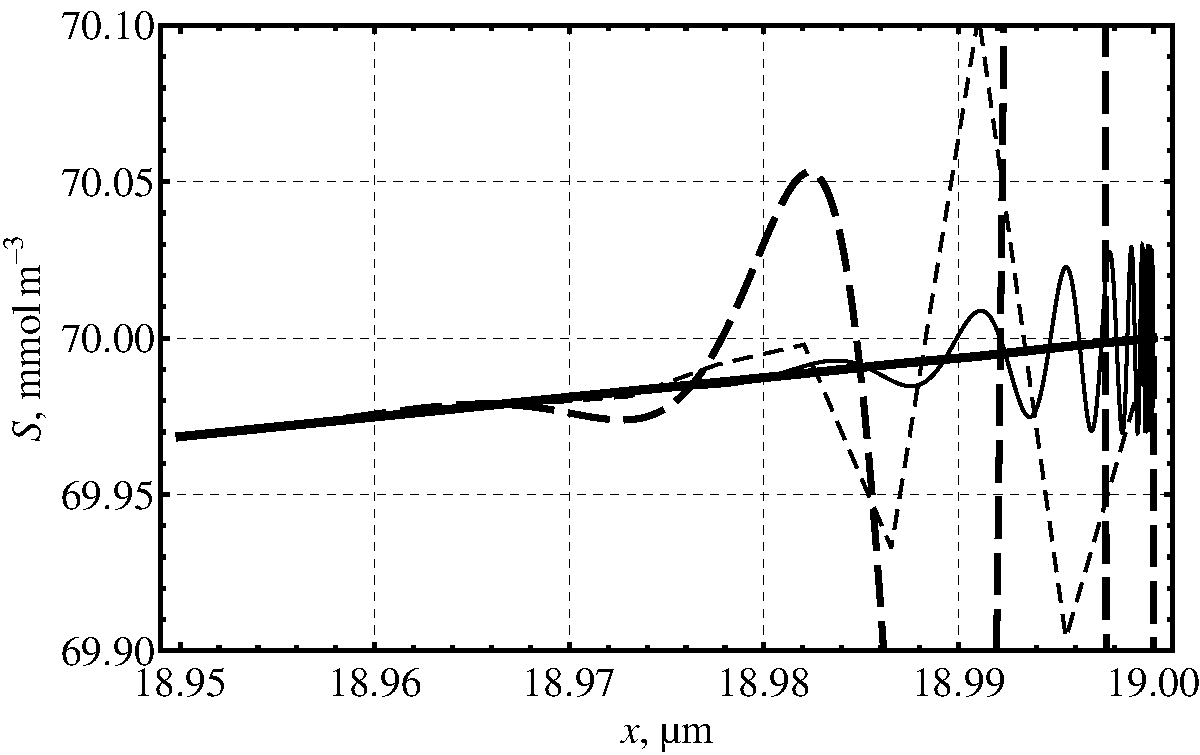
\includegraphics[clip=true, width=\textwidth]{Iliustracijos/Fig_Osciliacijos_Del_Netolygiu_Tinklu.pdf}\\
    The substrate concentration $S(x,t^*)$ vs the coordinate $x$ (near the point $x = d_e + d_m ={}$\SI{19}{\micro\metre}).
\end{minipage}
\;
\begin{minipage}{0.48\textwidth}
    \pause
    \begin{alertblock}{For best results we recommend to use uniform grid in coordinate direction and non-uniform (finer at the starting moment of modeling) grid in time direction.}
    \smallskip
    Otherwise -- expect some oscillatory artifacts (in the profile of substrate concentration) near boundary of the outer layer.
    Luckily, these artifacts do not appear in any other part of substrate or product concentration profiles, also, they do not propagate to the electrode,
    hence they have no effect on evaluation of biosensor response.
    \end{alertblock}
\end{minipage}
}

\end{frame}
%%%%%%%%%%%%%%%%%%%%%%%%%%

\subsection{Degradation impact on biosensor response}

%%%%%%%%%%%%%%%%%%%%%%%%%%
\begin{frame}[shrink=11]{Relative decay $\Delta I$ vs degradation rates $C_1$ and $C_2$}

\begin{exampleblock}{}
As a response of the electrochemical biosensor, a steady-state diffusion current density ($I$) on the electrode is considered.
\end{exampleblock}

Examine relative decay $\Delta I$ of biosensor response vs degradation rates $C_1$ and $C_2$:
\[
    \Delta I  =  \left( 1 - \frac{I\left( C_1, C_2 \right)}{I\left( 0, 0 \right)} \right) \cdot 100\%.
\]

\pause
\vspace*{-2mm}
\begin{block}{Graphical notations:}
\begin{itemize}

\item
a \emph{white region} correspond to the values of $C_1$ and $C_2$ such that $0\% \leqslant \Delta I \leqslant 1\%$;

\item
a \emph{criss-crossed region on a white background} -- such that $1\% \leqslant \Delta I \leqslant 2\%$;

\item
a \emph{light grey region} -- such that $2\% \leqslant \Delta I \leqslant 3\%$;

\item
a \emph{criss-crossed region on a light grey background} -- such that $3\% \leqslant \Delta I \leqslant 4\%$,

\end{itemize}
and so on.
\end{block}

\end{frame}
%%%%%%%%%%%%%%%%%%%%%%%%%%

%%%%%%%%%%%%%%%%%%%%%%%%%%
\begin{frame}{Relative decay $\Delta I$ vs degradation rates $C_1$ and $C_2$}

\centering{
\begin{minipage}{0.48\textwidth}
    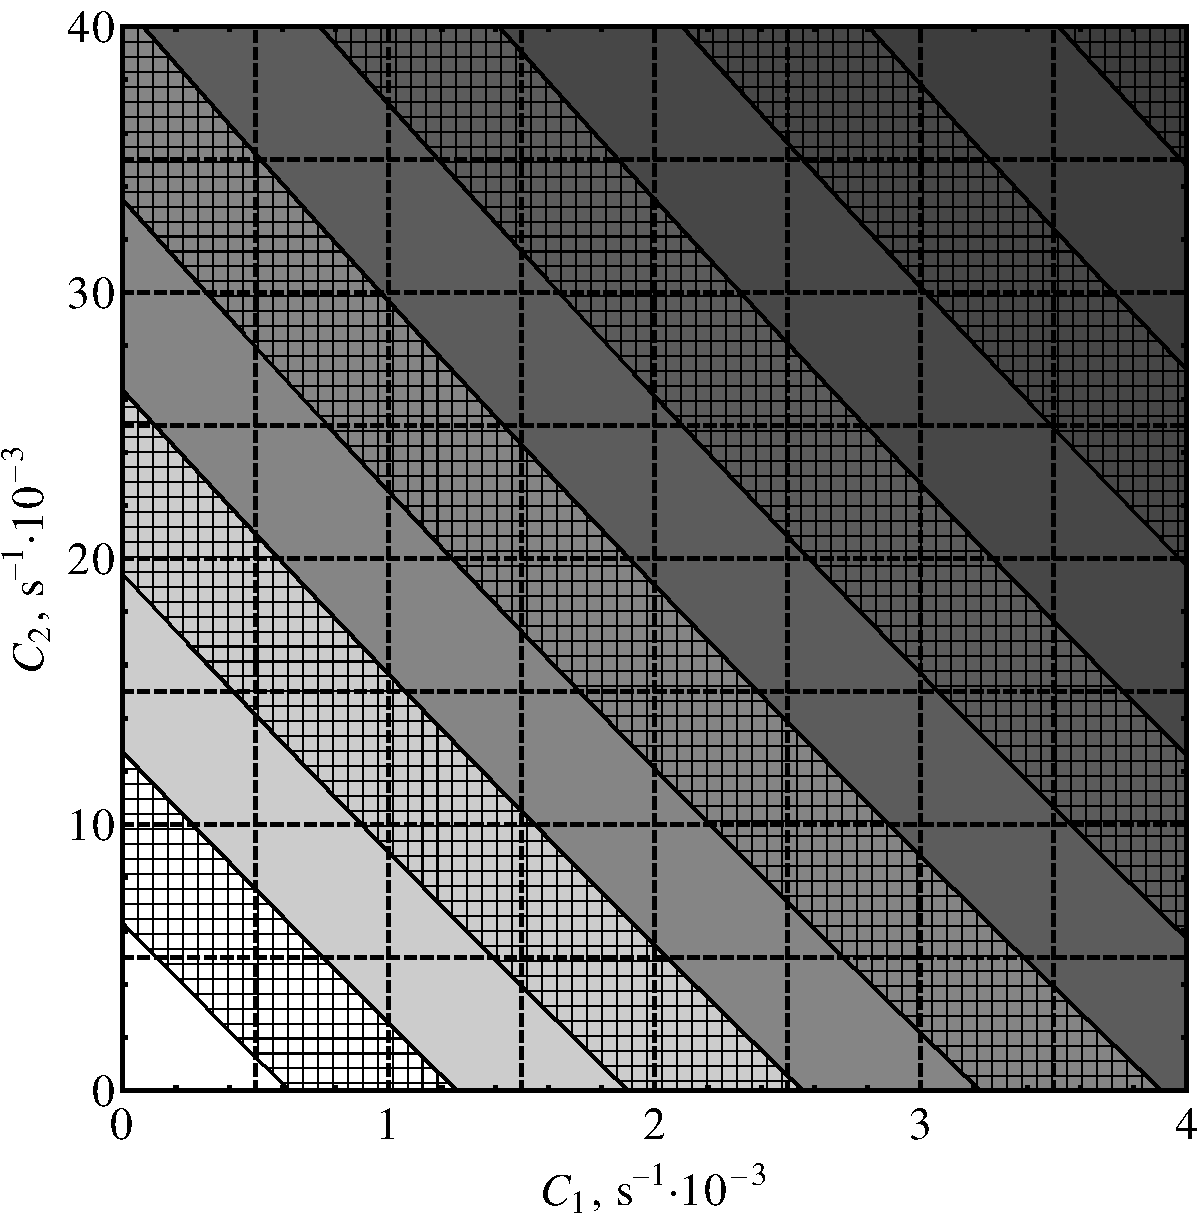
\includegraphics[clip=true, width=\textwidth]{Iliustracijos/Fig2a.pdf}\\
    The case when the product diffuses out of the biosensor.
\end{minipage}
\;
\begin{minipage}{0.48\textwidth}
    \smallskip
    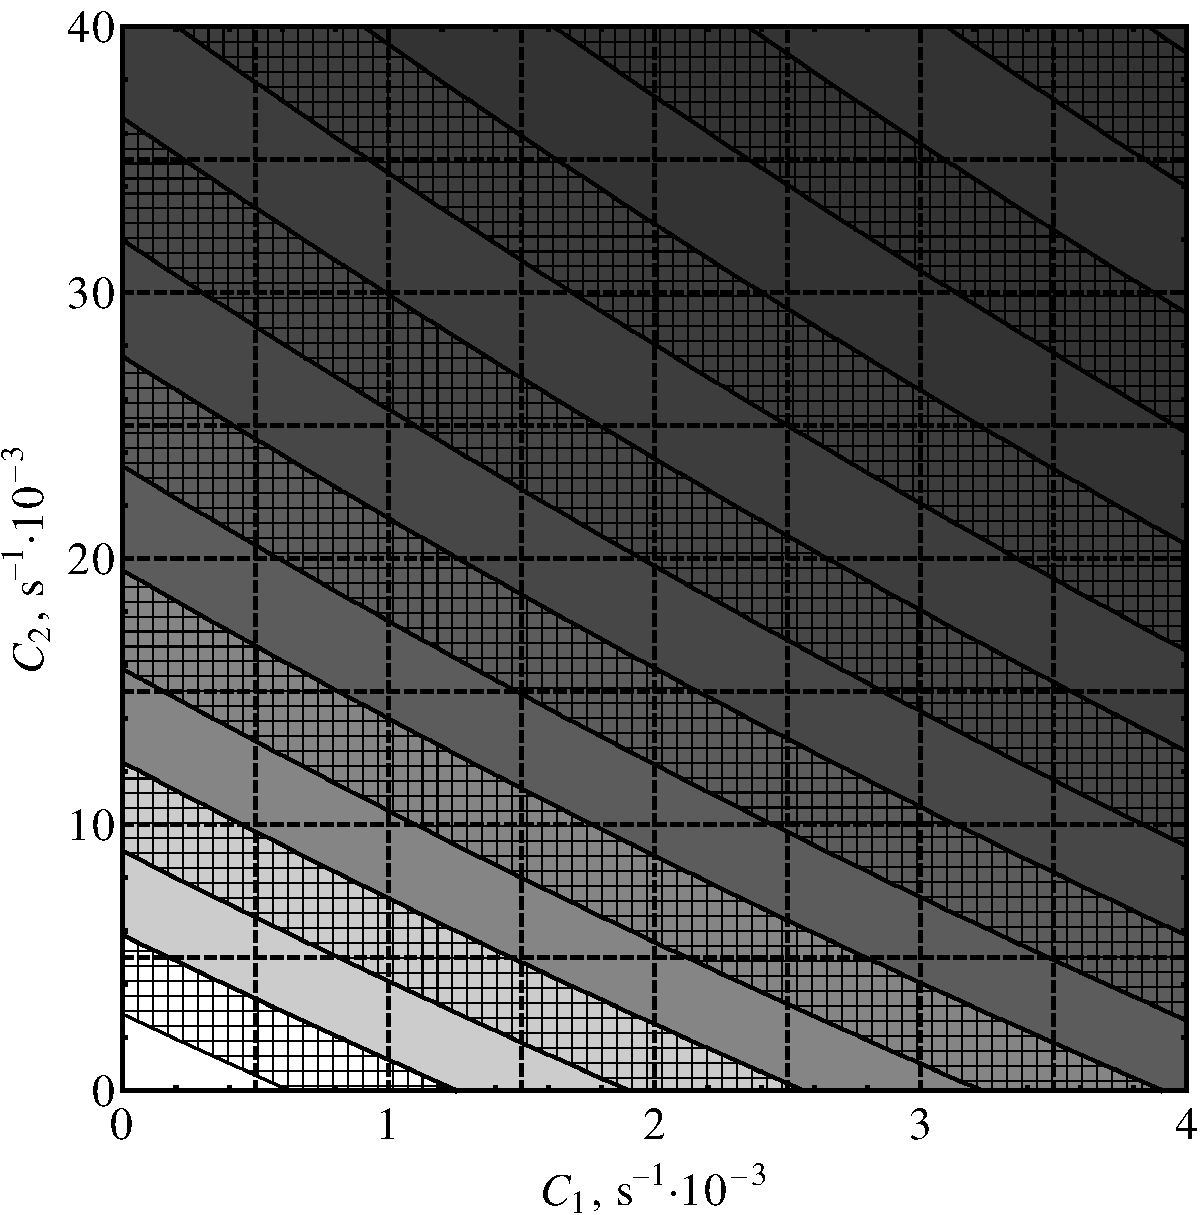
\includegraphics[clip=true, width=\textwidth]{Iliustracijos/Fig2b.pdf}\\
    The case when the outer membrane is impermeable for the product.
\end{minipage}
}

\end{frame}
%%%%%%%%%%%%%%%%%%%%%%%%%%

\subsection{Influence of outer membrane thickness}

%%%%%%%%%%%%%%%%%%%%%%%%%%
\begin{frame}{How would the varying thickness of the outer membrane influence the impact of the degradation process to the biosensor response?}

\begin{exampleblock}{}
In the analyzed model of the biosensor we have assumed that the thickness of the outer membrane is constant.
\end{exampleblock}

\pause
\begin{block}{}
However, in real situations this parameter may vary.

\smallskip
Cells and proteins from biological media can adsorb on surfaces of the outer membrane, ``gluing'' the outer membrane,
hence increasing the thickness of the outer membrane.

\smallskip
Also, the thickness of the outer membrane can be affected by pressure fluctuations of the bulk.
pH fluctuations can impact the swelling properties \textit{etc.}
\end{block}

\end{frame}
%%%%%%%%%%%%%%%%%%%%%%%%%%

%%%%%%%%%%%%%%%%%%%%%%%%%%
\begin{frame}[shrink=28]{Impact of outer membrane thickness on curve $\Delta I = 5$\%}

\begin{block}{Define the area in $\left( C_1, C_2 \right)$ coordinate plane, limited by $\Delta I$ $5$\% isoline:}
\vspace*{-4.5mm}
\[
    \Psi  =  \left\{ \left( C_1\geqslant 0, C_2\geqslant 0 \right): \Delta I \leqslant 5\% \right\}.
\]
\end{block}

\pause
\centering{
\begin{minipage}{0.48\textwidth}
    \smallskip
    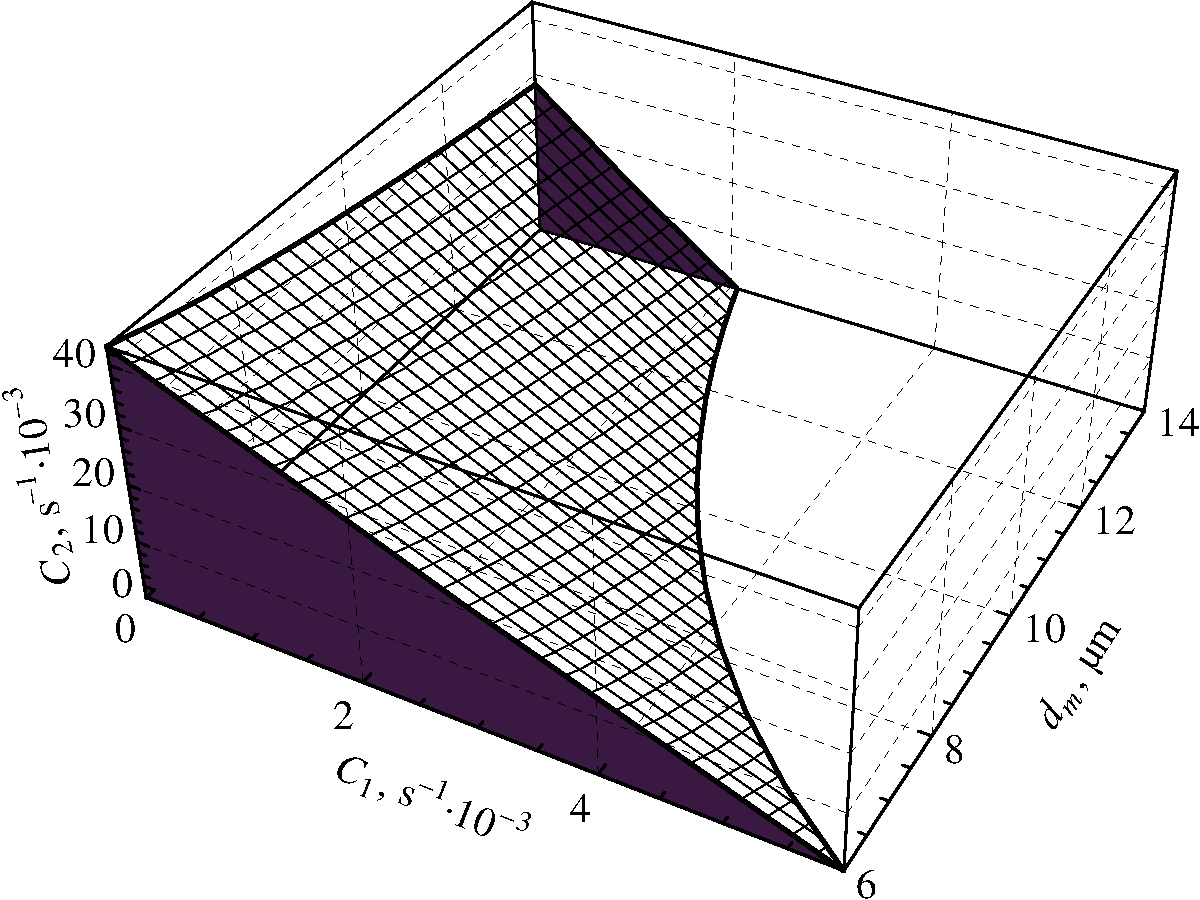
\includegraphics[clip=true, width=\textwidth]{Iliustracijos/Fig3.pdf}\\
    Dependency of the area $\Psi$ (displayed in dark gray background) on the outer membrane thickness $d_m$.
    The case when the product diffuses out of the biosensor.
\end{minipage}
\;\;
\begin{minipage}{0.48\textwidth}
    \begin{exampleblock}{\emph{The analytical} approximation of the curve $\Delta I = 5$\%}
    By employing least squares fitting we have obtained the analytical formulae
    \begin{alignat*}{1}
        & C_2  =  K\!\left( d_m \right) C_1  +  M\!\left( d_m \right), \\
        & K\!\left( d_m \right)  =  -0.792\, \frac{d_m}{\si{\micro\metre}}  -  2.49, \\
        & M\!\left( d_m \right)  =  \frac{ \displaystyle -0.583\, \frac{d_m}{\si{\micro\metre}}  +  28.3  +
            \frac{\SI{110}{\micro\metre}}{d_m} }{ \displaystyle 10^3 }\, \si{\per\second}.
    \end{alignat*}
    \end{exampleblock}
\end{minipage}
}

\end{frame}
%%%%%%%%%%%%%%%%%%%%%%%%%%

\subsection{Influence of substrate concentration}

%%%%%%%%%%%%%%%%%%%%%%%%%%
\begin{frame}[shrink=24]{Impact of substrate concentration on curve $\Delta I = 5$\%}

\centering{
\begin{minipage}{0.48\textwidth}
    \smallskip
    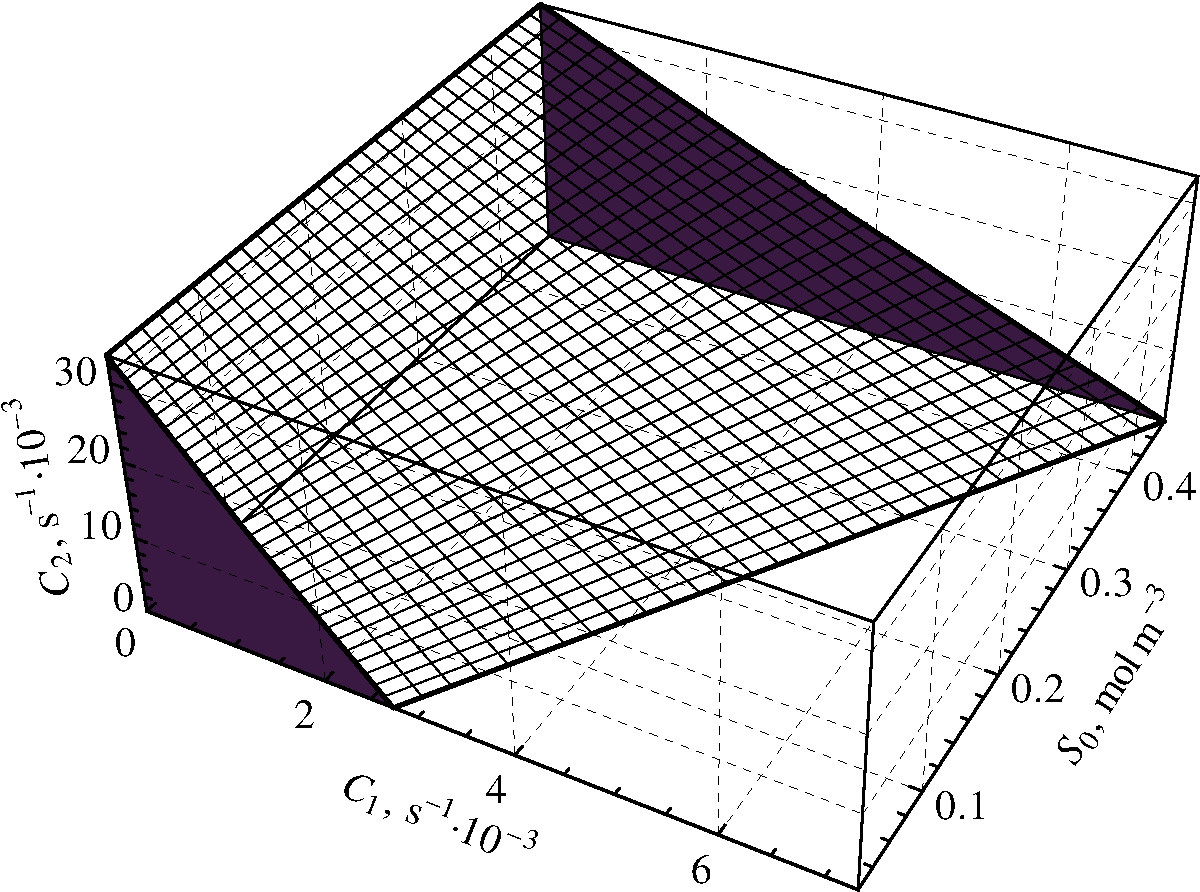
\includegraphics[clip=true, width=\textwidth]{Iliustracijos/Fig4.pdf}\\
    Dependency of the area $\Psi$ on the substrate concentration $S_0$ in buffer solution.
    The case when the product diffuses out of the biosensor.
\end{minipage}
\;\;
\begin{minipage}{0.48\textwidth}
    \begin{exampleblock}{\emph{The analytical} approximation of the curve $\Delta I = 5$\%}
    Least squares fitting yields the analytical formulae
    \begin{alignat*}{1}
        & C_2  =  k\!\left( S_0 \right) C_1  +  m\!\left( S_0 \right), \\
        & k\!\left( S_0 \right)  =  -\,\frac{33.5}{10.5\, S_0\, \si{\per\mole\metre\cubed}  +  2.49}, \\
        & m\!\left( S_0 \right)  \equiv  \SI{0.0335}{\per\second}.
    \end{alignat*}
    \end{exampleblock}
\end{minipage}
}

\pause
\begin{alertblock}{}
Also we have analyzed situation with different $V_{max}$.

This analysis shows that activity of the biocatalyser does not influence the impact of the degradation processes on the biosensor response. 
\end{alertblock}

\end{frame}
%%%%%%%%%%%%%%%%%%%%%%%%%%

%%%%%%%%%%%%%%%%%%%%%%%%%%%%%%%%%%%%%%%%%%%%%%%%%%%%%%%%%%%%%%%%%%%%%%%%%%%%%%%%
\section{Conclusions}
%%%%%%%%%%%%%%%%%%%%%%%%%%%%%%%%%%%%%%%%%%%%%%%%%%%%%%%%%%%%%%%%%%%%%%%%%%%%%%%%

%%%%%%%%%%%%%%%%%%%%%%%%%%
\begin{frame}{Conclusions}

\begin{block}{}
\begin{itemize}

\item
The Crank--Nicolson method for numerical modeling of a multilayer electrochemical biosensor,
may produce some oscillatory artifacts (in the profile of substrate concentration) near boundary of the outer layer.
Luckily, these artifacts do not appear in any other part of substrate or product concentration profiles, also, they do not propagate to the electrode of the biosensor,
hence they have no effect on evaluation of biosensor response.
To avoid such artifacts,
we recommend to use \emph{uniform grid in coordinate direction} (other bonuses of such decision are decreased time of computations and simpler implementation)
and \emph{non-uniform (finer at the starting point $t=0$) grid in $t$ direction}.

\end{itemize}
\end{block}

\end{frame}
%%%%%%%%%%%%%%%%%%%%%%%%%%

%%%%%%%%%%%%%%%%%%%%%%%%%%
\begin{frame}[shrink=21]{Conclusions}

\begin{block}{}
\begin{itemize}

\item
When the product diffuses out of the biosensor, the response is more sensitive to the degradation process of the substrate (compared to the degradation of the product).
That is, the same value of the response decay would be achieved with the substrate degradation (assumed the product does not degrade) rate approximately $10$ times lesser
than the product degradation.

\pause
\smallskip
\item
If the outer membrane is impermeable for the product (the product is trapped inside the biosensor), the impact of the substrate degradation is the same as in the previous case,
but the biosensor becomes more sensitive to the rate of the product degradation.

\pause
\smallskip
\item
When the thickness of the outer membrane increases, the degradation processes become more influential.
With increase of substrate concentration, the substrate degradation rate (needed for the same value of the response decay) increases linearly.
The activity of the biocatalyser does not influence the impact of the degradation processes on the biosensor response.

\pause
\smallskip
\item
Analytical formulae, relating the degradation rates and the outer membrane thickness or the initial substrate concentration have been obtained.
These findings can be included into a biosensor monitoring algorithm, as correction of allowed limit of the biosensor response.

\end{itemize}
\end{block}

\end{frame}
%%%%%%%%%%%%%%%%%%%%%%%%%%

%%%%%%%%%%%%%%%%%%%%%%%%%%
\begin{frame}{Thank You for Your attention!}

\centering{{\Large Any questions, please?}}

\end{frame}
%%%%%%%%%%%%%%%%%%%%%%%%%%

\end{document}

